\documentclass[journal]{IEEEtran}
\usepackage[utf8]{inputenc}

\usepackage[sorting=none]{biblatex}
\usepackage{graphicx}

\addbibresource{bibliography.bib}

\begin{document}

    \markboth{Cybersecurity :Analysis of  Attack forecasting, January~2021}%
{cyber Security :Analysis of  Attack for-casting, January~2021}

\title{Cybersecurity : Analysis of  Attack forecasting}
\author{Tomás O'Malley,~\IEEEmembership{ BSc Software Development (Honours),~GMIT}%
}
% Author: Tomás O'Malley G00361128 @ gmit.ie
% Student of Galway-Mayo Institute of Technology, Department of Computer Science and Applied Physics
% Literature Review on Cyber Security completed as part of Research Methods in Computing and IT weight:70%.

\maketitle

\begin{abstract}
Abstract—This review will tackle and review the current state of cyber-security and forecasting models developed. Computers have become the foundation and backbone of how we communicate, interpret data, and push forward today. Over the last decade advancements in information technology from the large consumer use of personal computers and smartphones have led to increased demand for tight security solutions in areas like e-commerce, social media sites, and including banking. Today ina society where big-data companies hold so much of our value-able data using cloud computing, IoT security, companies must provide high-level security to prevent attacks on their customers and income. I later in this review, discuss the current state of cyber security forecasting and future gaps/advancements through the use of deep learning and artificial intelligence.



\end{abstract}
\begin{IEEEkeywords}
cybersecurity, information  technology, cloud-computing, attack-forecasting, deep learning

\end{IEEEkeywords}

\section{Introduction}


\subsection{A Brief History of Cyber Security}
As far back as the early 1970s cybersecurity has been a prevailing topic in society beginning with the ARPANET (The Advanced Research Projects Agency Network)\cite{Arpanet}. By nature humans and their systems are flawed, threats such as Malware, Phishing, Trojans,  DDoS still exist today. Data breaches such as the  Bright Researchers have been brewing algorithms to prevent cybercrimes (Identity fraud,  card payment data). Information technologies and the introduction to Tim Berners Lee Wide Wide Web in 1989 added a new layer of threats for governing groups using AV technology and firewalls to force restrictions from specified network access. New obstacles include the introduction of ransomware in 2017 forcing windows users to pay to gain access to their device. As described by the multinational company in the year of 1991  \cite{consumer}" Less than a year after SAM and Norton Utilities came together, Symantec launched Norton AntiVirus™ for PC — its very first antivirus software for consumers" continue to provide security options in 2020. Underneath is a Gantt chart provided.




\subsection{Current state of security} \label{subsec:Computing}

When viewing cybersecurity there are three main trends for gateways for malicious attacks CNA-Computer Network Attack, CNE-Computer network Exploitation, and CNI-Computer Network influence, Cyber Crimes are prevailing and \cite{crime} Europol states that cyber crimes have now become more common than street crime. Research firm Juniper claim \cite{iotStatistics} "IoT connections to grow  140 percent to hit 50 billion by the year  2022, as edge computing accelerates ROI".Due to the covid-19 pandemic (2020) currently employees globally are working remotely to maintain and improve fault tolerance services. New data shows the pandemic will benefit but deeply challenge cybersecurity and how companies fund services. Microsoft has issued a statement \cite{microsoft} "Technology alone cannot keep pace with the threats and demands facing businesses and their largely remote workforces." 



\begin{figure}[h]
\centering
{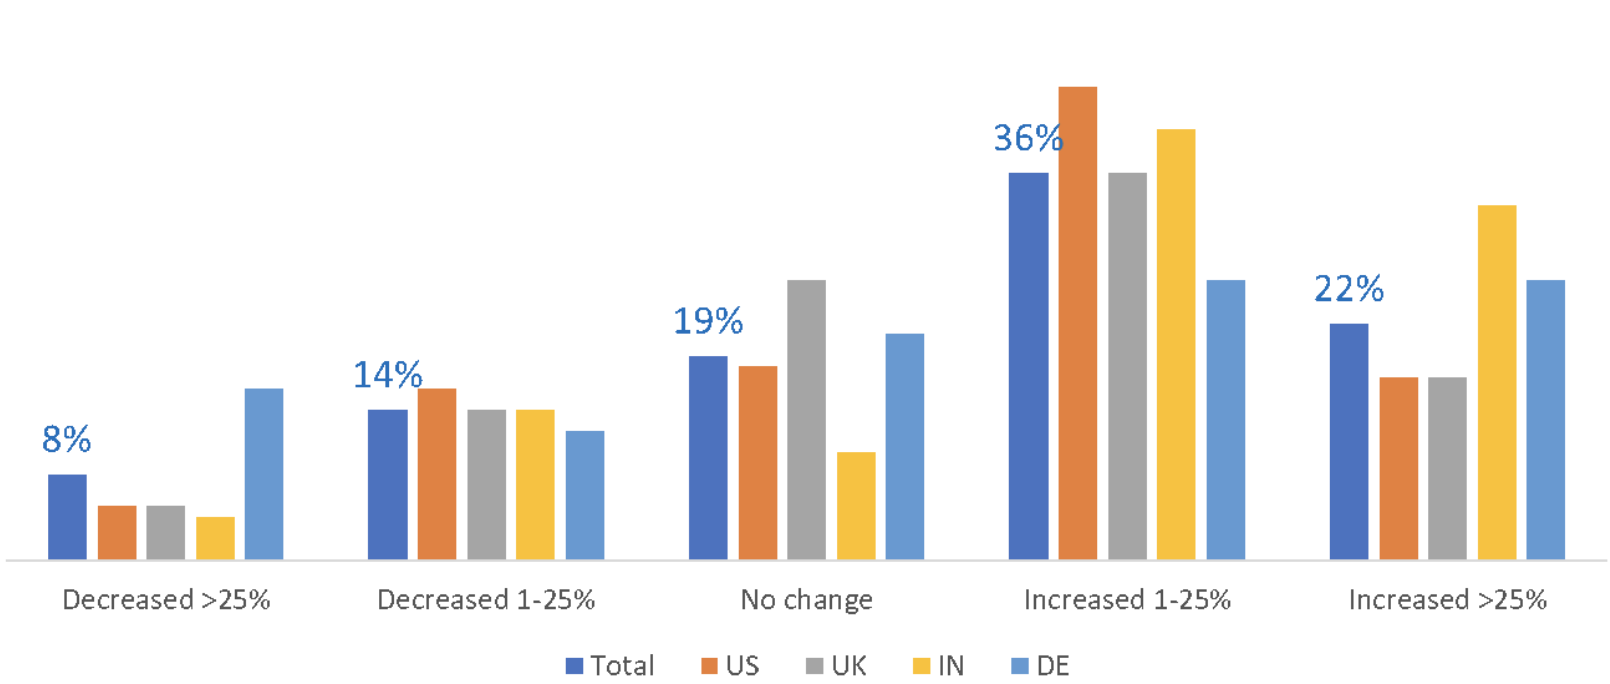
\includegraphics[width=.45\textwidth]{LiteratureReviewAttackForecasting/Other/photos/responsetoPandemic.png}}

\caption{ Fig.1 2020 pandemic Multinational  budget changes }

\end{figure}





\section{Solutions}


\subsection{The Definition of Cyber Security}

Cybersecurity is described in websters dictionary as " measures taken to protect a computer or computer system (as on the Internet) against unauthorized access or attack".  It's also known as information technology security or electronic information security. The term applies in a variety of contexts, from business to mobile computing, and can be divided into a few common categories. From military research, a methodology referred to as cyber situational awareness is applied. One of the most widely used definitions of situational awareness is by Endsley  in their paper \cite{situationalAwareness} “Perception
of the elements in the environment within a volume of time and
space, the comprehension of their meaning, and the projection
of their status in near future.” 




\label{subsec:cyberattacks}
As of 2018, there have been 80,000 cyberattacks a day, The key is for Big-data companies to develop a threat model in which these threats can be pre-determined and dealt with in advance.




%\textsc{1) Attack Forecasting : }
\subsubsection{Attack Forecasting}
Attack forecasting in principle can be compared to the benefits of the weather forecast so we can prevent/dodge an unwanted position. Quantum cryptography is the science of exploiting quantum mechanical properties to perform cryptographic tasks. The best-known example of quantum cryptography is the quantum key distribution which offers an information-theoretically secure solution to the key exchange problem. As touched on by Martin Husak \cite{attackForecasting} we must to document the behavior of the attackers and establish a description of an attack for later use when incorporated into a realistic model. An adaption commonly used is the "Hidden Markov Models states for prediction" outlined in Alireza paper \cite{prediction}. By observing and analyzing the attempts we can forecast future events as described by \cite{hmmn} "allows us to talk about both observed events Hidden Markov model that we think of as causal factors in our probabilistic model of observable events".\cite{modelDefinition}
The Hidden Markov model was first used in speech recognition and has been successfully applied to the analysis of biological sequences since late 1980 in computing.

\begin{figure}[h]
\centering
{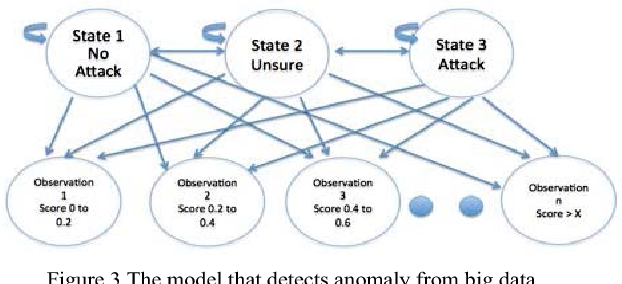
\includegraphics[width=.45\textwidth]{LiteratureReviewAttackForecasting/Other/photos/hiddenmark.png}}



\caption{ Fig 2 provides an application of a The Hidden Markov Model. }

\end{figure}
The model focuses on three states. 

\begin{itemize}
  \item State 1 No  Attack  : state in which the service has not been attacked. 
  \item State 2 Unsure : state in which there is potential of further attack.
\item State 3   Attack : state in which the organisations services have experienced unexpected/unusual traffic.

\end{itemize}



%\textsc{3) Research and Development : }
\subsubsection{Types of Attacks }
Cyber attacks have been a serious computing issue since the dawn of computing from the floppy disk to over networks.There are many methods and classifications of threats for online security. Underneath I will evaluate the most common threats faced by governed data and consumer data.Documentation from CSI Computer Crime & Security Survey \cite{csiSurvey}


\begin{enumerate}
  \item     Virus: Alison Grace for Norton security \cite{nortonVirus}  describes a virus as an "A computer virus, much like a flu virus, is designed to spread from host to host and has the ability to replicate itself. "
    \item    Phishing: As defined by websters dictionary ": a scam by which an Internet user is duped (as by a deceptive e-mail message) into revealing personal or confidential information which the scammer can use illicitly".Prime examples of phising can be found in your email client sometimes in the form of spam requesting information.

  \item     Denial of Service (DDOS): As described by Steve Weisman team at Norton \cite{nortonSecurity} "Distributed denial-of-service attacks target websites and online services. The aim is to overwhelm them with more traffic than the server or network can accommodate. The goal is to render the website or service inoperable."DDOS attacks take advantage off less secure architecture.
  
  


\end{enumerate}

These are all prime examples of modern-day cyber threats that companies must prepare to prevent

\section{Proposed Technologies}

With three fundamental motivations behind Cyber Security in mind, we must then contemplate the technologies required to achieve such goals. Like its standards, cyber attack technologies have also not been completely decided on. However, some promising technologies have emerged and include; Blockchain, Model Development, and Deep Learning.


\subsection{Blockchain}\label{subsec:Blockchain}
Blockchain technology enables trusted transactions among untrusted participants in the network. Incorporating the blockchain completely eliminates the need for businesses to authenticate and provide secure access to users and devices without using any password. Blockchain technologies were invented in the year 2009 created to replace flat currency and currently, there are few literature reviews due to its short introduction in security. As of last (2019) year, a paper by Salman \cite{blockchainSurvey} discusses  "The technology
started with Bitcoin, a cryptocurrency that has reached a capitalization of 180 billion dollars as of January 2018".Currently in the market their seems to be large investment and research for blockchain in digital currency and a gap in research for addition to cyber-threat and attack forecasting.

 
\subsection{Big Data
}\label{subsec:BigData}
Websters Dictionary defines big-data as an accumulation of data that is too large and complex for processing by traditional database management tools. Examples of sources of big data
transactions are data from computer networks,
telecommunication networks ( BT, Verizon, finance (Fidelity, healthcare (HSE), social media (Google+), etc. The domain of Big Data Analytics (BDA) is concerned with the
extraction of value from big data, i.e., insights that are nontrivial, previously unknown, implicit, and potentially useful. Seagate the multinational store 75 zettabytes(. One Zettabyte is approximately equal to a thousand Exabytes, a billion Terabytes, or a trillion Gigabytes)  of data by the year 2025.



The act of accessing and storing large amounts of information for analytics has been around for a long time. By optimizing/surveying pools of data companies can try to forecast the next attempt. In A. Gheyas survey   \cite{surverydata}  He outlines The key challenges facing the insider threat detection and prediction system include unbounded patterns, It is extremely difficult to harvest the data correctly and model for the behavior to prevent attacks from the model created.


\subsection{Develop Model}
The aim is to create impact solutions rather than point fixes for large scale systems.

%\dddd. train model
Xing describes the training as a model for predicting attacks In the training process, we use the mini-batch gradient descent method to compute the minimum of the objective function, which is described in Eq. (1). We use 10,000 iterations to train a network and set the penalty parameter λ =.001 because other parameters do not lead to any significantly better results. For each dataset, we use Algorithm 1 to compute the fitted values with varying model parameters. We select the model that achieves the minimum MSE.\cite{trainModel} 

It is a common construction for companies to create state cycles as reviewed in the journal .



\subsection{Deep Learning}\label{subsec:Deep-Learning}

Deep learning refers to a type of machine learning based on artificial neural networks in which multiple layers of processing are used to extract progressively higher-level features from data. As outlined by Vinayakumar the raw input can be applied towards use cases such as intrusion detection, malware classification.There a many approaches for deep learning such as Recurrent neural network (RNN) , Long Short Term Memory Networks(LSTMN's) and Self Organizing Maps (SOMs).Deep learning is incorporated into many types of security software used by both consumers and organisations.Organisations will need to train the model by using their own data set to create predictions for the possibilities of an attack to their services.




\cite{security} 


\section{The Future of  Cyber Security}


\subsection{Emerging threats in  Cyber Security}
Complications and questions arise with each major development in any area of online technologies.


\subsubsection{Ever Expanding Users  }
%\textsc{1) Ever Expanding Users: }
As of the year 2020, there are 1.69 billion users on the social media platform "Facebook" standalone. Through the ever-expanding of the used Internet of things and smart devices leads to more potential attacks to their data. Each decade a new platform succeeds the last from MySpace to Facebook. Companies must incorporate solutions to prevent intrusions on all devices such as  Android, PC, Mac, and iOS.Due to the Covid-19 Pandemic Students are learning completely in a digital format vulnerable to attacks such as Phishing, Malware, DDoS ( Direct Denial of Service), and Ransomware. 


%\textsc{2) Social Engineering: }
\subsubsection{Social Engineering}
Websters Dictionary defines social engineering as ": management of human beings in accordance with their place and function in society : applied social science".In recent years juggernaut company yahoo in 2013 was attacked which resulted in a breach of 3 billion accounts holding names, passwords, and card data due to the use of social engineering from an outside entity.It is very difficult to element this factor as it is entirely human dependent.

\subsection{Possible Use Cases of Attack  Forecasting in 
Cyber  Security}
In a world where Big Data becomes more sophisticated and unpredictable by the day in this section, I will define and outline the 3 possible use cases in Attack forecasting systems.
\subsubsection{In Day-to-Day  Life}
One of the largest advantages of attack forecasting is from the user's endpoint. If Multinational-companies such as Google Microsoft, Apple successfully crack the code user downtime will be lowered and create a stronger dependence and trust for organizations and consumers. An example of a company attacked using DDOS is Sony, The attack occurred between April 17 and April 19, 2011, forcing Sony to turn off the PlayStation Network on April 20, This large outage has had dire consequences for its brand reputation and users faith in their security.

\subsubsection{The Bigger Picture}
The leap from current computing to the fifth generation(Quantum Computing)of computing will allow for the creation of quantum-safe encryption in cryptography.It  is undeniable that  user experience on many levels can  be greatly improved. However, it is important to recognise the benefits of improved  cybersecurity on a societal and global level.In education, one large advantage of attack-forecasting is the reduction of down times for multimedia platforms for connecting eachother. Additionally attack forecasting can provide higher reliability/dependence to pave the path for smart cities and autonomous transport .

\section{Conclusion}
The way we communicate and incorporate technology into both our personal lives and wider society is changing greatly with each passing year. While the technologies mentioned in this review have shown considerable potential, but there is yet much research and landmarks to overcome before attack forecasting can change  Security  for consumers and developers.These possibilities, coupled with the need to improve on  current cybersecurity systems and our ever-increasing demand for higher 24/7 365 services no downtime and more reliable systems, will be the driving forces behind the advancements to come in the future.



\bigskip
\bigskip

\printbibliography
\end{document}